\documentclass[12pt, a4paper]{article}
\usepackage{amsmath, amssymb, amsthm, mathtools, graphicx, slashed}
\usepackage{subcaption}%Permet d'utiliser subfigure
\usepackage[top=1cm, bottom=1.5cm, left=1cm, right=1cm]{geometry}
\usepackage[compat=1.1.0]{tikz-feynman}
\usepackage{verbatim}
\usepackage{hyperref}
%\tikzfeynmanset{compat=1.1.0}
\title{Devoir de BSM du 09 Juin 2026 }
\author{RAZAFIMAHERY Faneva Liantsoa\\ 
 	\small{Master 2- Physique des Hautes Energies} \\ \small{Université d'Antananarivo}}
\date{\small 12 Juin 2026}
 \begin{document}
 	\maketitle
 	\begin{abstract}
 		\textit{Dans ce travail, il nous a été demandé de trouver l'amplitude de l'interaction suivante: à l'entrée un quark ($q$) et un gluon ($g$) et à la sortie un quark ($q$) et un gluon ($g$), c'est-à-dire $\mathcal{M}(q+g \rightarrow q+g)$.\\
 		Celà grâce aux règles de Feynman habituelles et sans utiliser le formalisme d'hélicité spinorielle développé en cours.}
 	\end{abstract}
 	\section*{Les règles de Feynman}
 	Dans ce qui suit, nous utilisons les règles de Feynman dans le document \cite{Cacciari} qui lui même cite \cite{Peskin:1995ev}.\\ % Mila MBOLA ATAO ANATY BIO...https://www.lpthe.jussieu.fr/~salam/teaching/M2-2009/FeynmanRules.pdf
 	Pour les éléments externes:
 	\begin{figure}[h]
 	\centering
 	 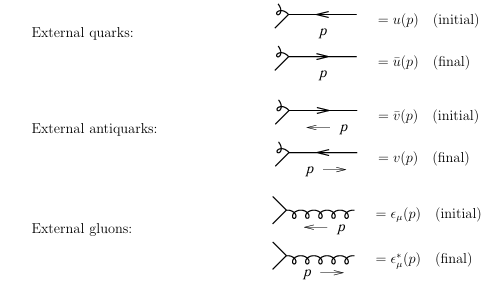
\includegraphics[width= 0.5\textwidth, height=5cm]{External}
 	\end{figure}\\
 	Et pour les élements internes:
 	\begin{figure}[htbp]
 		\begin{subfigure}{0.5\textwidth }
 		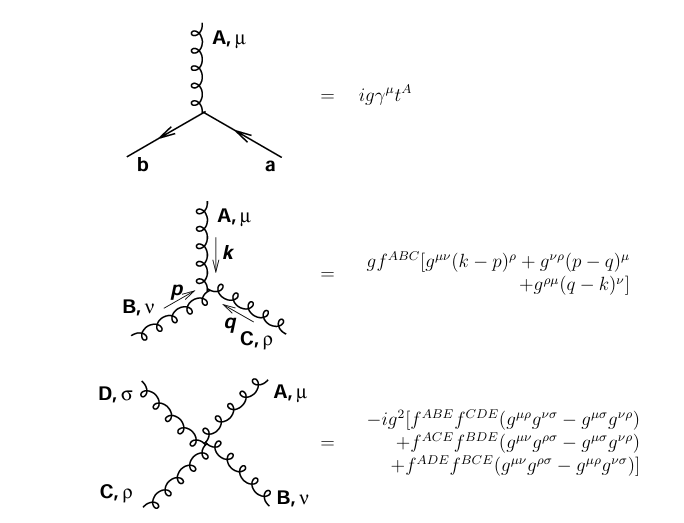
\includegraphics[height=7cm]{Internal1}
 		\end{subfigure}		
 		\begin{subfigure}{0.5\textwidth}
 		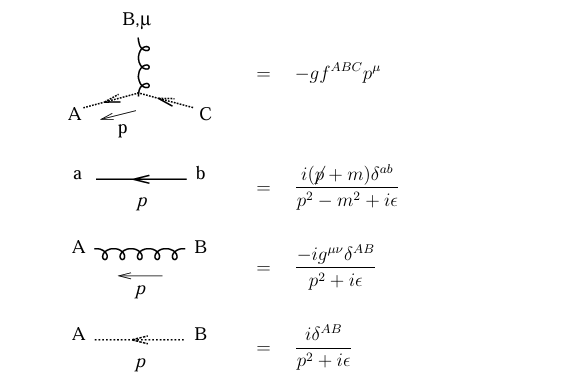
\includegraphics[height=7cm]{Internal2}
 		\end{subfigure}
 	\end{figure}
 	\newpage
 	%\section*{Le lagrangien avec interaction quark-gluon}
 	%Rappelons aussi que le lagrangien qui nous permet d'avoir les termes d'interactions possibles s'écrit comme suit:
 	\section*{Les diagrammes possibles}
 	Grâce aux règles de Feynman, nous voyons qu'il n'y a que trois diagrammes de Feynman  possibles pour cette interaction:
 		%\usepackage[utf8]{inputenc}
 		\begin{comment}
 		\begin{figure}[htbp]
 			\centering
 			
 			% s channel
 			\begin{minipage}{0.32\textwidth}
 				\centering
 				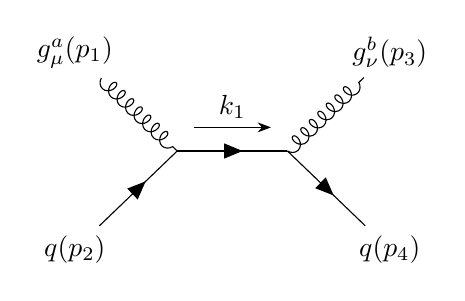
\begin{tikzpicture}[baseline=(v1)]
 					\begin{feynman}
 						% External Nodes
 						\vertex (i1) at (0, 2.5) {\(g^a_\mu(p_1)\)};
 						\vertex (i2) at (0, 0)   {\(q(p_2)\)};
 						\vertex (o1) at (4, 2.5) {\(g^b_\nu(p_3)\)};
 						\vertex (o2) at (4, 0)   {\(q(p_4)\)};
 						
 						% Internal Vertices with Lorentz/Color labels
 						\vertex (v1) at (1.3, 1.25); %[label=above left:{\(\mu, a\)}];
 						\vertex (v2) at (2.7, 1.25); %[label=above right:{\(\nu, b\)}];
 						
 						% Connections
 						\diagram* {
 							(i2) -- [fermion] (v1),
 							(i1) -- [gluon] (v1),
 							(v1) -- [fermion, momentum=\(k_1\)] (v2),
 							(v2) -- [fermion] (o2),
 							(v2) -- [gluon] (o1),
 						};
 					\end{feynman}
 				\end{tikzpicture}
 				\caption{\(s\)-channel}
 			\end{minipage}
 			\hfill
 			% t channel
 			\begin{minipage}{0.32\textwidth}
 				\centering
 				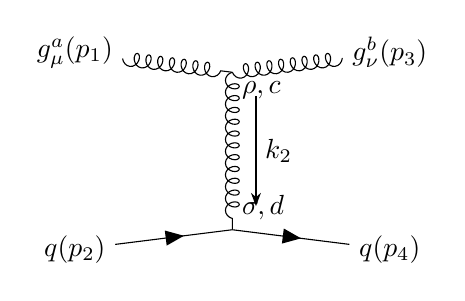
\begin{tikzpicture}[baseline=(v1)]
 					\begin{feynman}
 						% External Nodes
 						\vertex (i1) at (0, 2.5) {\(g^a_\mu(p_1)\)};
 						\vertex (i2) at (0, 0)   {\(q(p_2)\)};
 						\vertex (o1) at (4, 2.5) {\(g^b_\nu(p_3)\)};
 						\vertex (o2) at (4, 0)   {\(q(p_4)\)};
 						
 						% Triple-gluon vertex (top) and Quark-gluon vertex (bottom)
 						\vertex (v1) at (2, 2.25) [label=below right:{\(\rho, c\)}];
 						\vertex (v2) at (2, 0.25)   [label=above right:{\(\sigma, d\)}];
 						
 						% Connections
 						\diagram* {
 							(i1) -- [gluon] (v1),
 							(v1) -- [gluon] (o1),
 							(i2) -- [fermion] (v2),
 							(v2) -- [fermion] (o2),
 							(v1) -- [gluon, momentum=\(k_2\)] (v2), % k_2 = p_1 - p_3
 						};
 					\end{feynman}
 				\end{tikzpicture}
 				\caption{\(t\)-channel}
 			\end{minipage}
 			\hfill
 			% u channel
 			\begin{minipage}{0.32\textwidth}
 				\centering
 				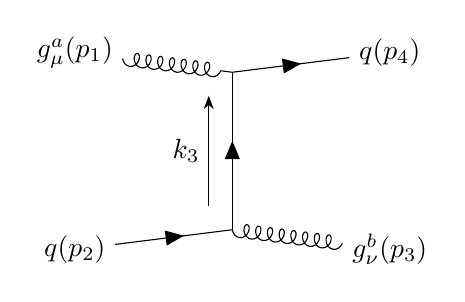
\begin{tikzpicture}[baseline=(v1)]
 					\begin{feynman}
 						% External Nodes
 						\vertex (i1) at (0, 2.5) {\(g^a_\mu(p_1)\)};
 						\vertex (i2) at (0, 0)   {\(q(p_2)\)};
 						\vertex (o1) at (4, 2.5) {\(q(p_4)\)};
 						\vertex (o2) at (4, 0)   {\(g^b_\nu(p_3)\)};
 						
 						% Triple-gluon vertex (top) and Quark-gluon vertex (bottom)
 						\vertex (v1) at (2, 2.25) ;%[label=below right:{\(\rho, c\)}];
 						\vertex (v2) at (2, 0.25)  ;% [label=above right:{\(\sigma, d\)}];
 						
 						% Connections
 						\diagram* {
 							(i1) -- [gluon] (v1),
 							(v1) -- [fermion] (o1),
 							(i2) -- [fermion] (v2),
 							(v2) -- [gluon] (o2),
 							(v2) -- [fermion, momentum=\(k_3\)] (v1), % k_2 = p_1 - p_3
 						};
 					\end{feynman}
 				\end{tikzpicture}
 				\caption{\(u\)-channel}
 			\end{minipage}
 			
 		\end{figure}
 	\end{comment}
 	
 	\begin{figure}[htbp]
 		\centering
 		
 		% s channel
 		\begin{minipage}{0.40\textwidth}
 			\centering
 			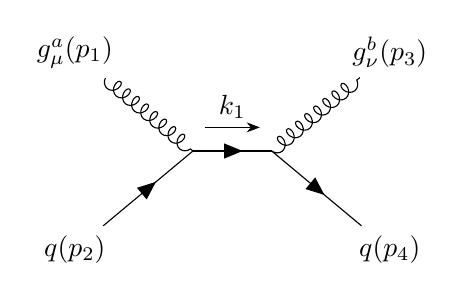
\begin{tikzpicture}[baseline={(current bounding box.center)}]
 				\begin{feynman}
 					% External Nodes
 					\vertex (i1) at (0, 2.5) {\(g^a_\mu(p_1)\)};
 					\vertex (i2) at (0, 0)   {\(q(p_2)\)};
 					\vertex (o1) at (4, 2.5) {\(g^b_\nu(p_3)\)};
 					\vertex (o2) at (4, 0)   {\(q(p_4)\)};
 					
 					% Internal Vertices
 					\vertex (v1) at (1.5, 1.25);
 					\vertex (v2) at (2.5, 1.25);
 					
 					% Connections
 					\diagram* {
 						(i2) -- [fermion] (v1),
 						(i1) -- [gluon] (v1),
 						(v1) -- [fermion, momentum=\(k_1\)] (v2),
 						(v2) -- [fermion] (o2),
 						(v2) -- [gluon] (o1),
 					};
 				\end{feynman}
 			\end{tikzpicture}
 			\caption{canal \(s\)}
 		\end{minipage}%
 		\begin{minipage}{0.55\textwidth}
 			\centering
 			\[
 			i\mathcal{M}_s = \bar{u}(p_4) \left( ig \gamma^\nu T^b \right) \frac{i \slashed{k}_1}{k_1^2 + i\epsilon} \left( ig  \gamma^\mu T^a \right) u(p_2) \,\epsilon_\mu(p_1) \epsilon_\nu^*(p_3)
 			\]			
 		\end{minipage}
 		
 		\vspace{1.5cm} % Espace vertical entre les lignes
 		
 		% t channel
 		\begin{minipage}{0.40\textwidth}
 			\centering
 			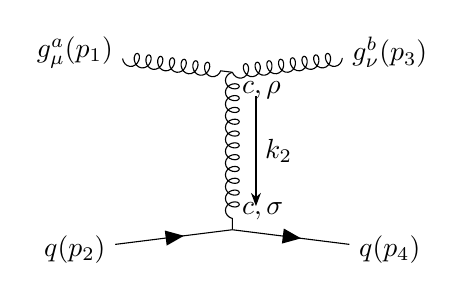
\begin{tikzpicture}[baseline={(current bounding box.center)}]
 				\begin{feynman}
 					% External Nodes
 					\vertex (i1) at (0, 2.5) {\(g^a_\mu(p_1)\)};
 					\vertex (i2) at (0, 0)   {\(q(p_2)\)};
 					\vertex (o1) at (4, 2.5) {\(g^b_\nu(p_3)\)};
 					\vertex (o2) at (4, 0)   {\(q(p_4)\)};
 					
 					% Triple-gluon vertex (top) and Quark-gluon vertex (bottom)
 					\vertex (v1) at (2, 2.25) [label=below right:{\( c,\rho\)}];
 					\vertex (v2) at (2, 0.25) [label=above right:{\(c,\sigma \)}];
 					
 					% Connections
 					\diagram* {
 						(i1) -- [gluon] (v1),
 						(v1) -- [gluon] (o1),
 						(i2) -- [fermion] (v2),
 						(v2) -- [fermion] (o2),
 						(v1) -- [gluon, momentum=\(k_2\)] (v2),
 					};
 				\end{feynman}
 			\end{tikzpicture}
 			\caption{canal \(t\)}
 		\end{minipage}%
 		\begin{minipage}{0.55\textwidth}
 			\centering
 			\begin{equation*}
 				\begin{split}
 					i\mathcal{M}_t =& \bar{u}(p_4) \left( ig  \gamma^\sigma T^c \right) u(p_2) \frac{-ig_{\sigma\rho}}{k_2^2 + i\epsilon} \\
 					&\times g f^{abc} 
 					[g^{\mu \nu}(p_1 -p_3)^{\rho}+g^{\nu \rho}(p_3 -k_2)^{\mu}+g^{\rho \mu}(k_2 -p_1)^{\nu}] \\
 					&\times \epsilon_\mu(p_1) \epsilon_\nu^*(p_3)
 					%C^{\mu\nu\rho}(p_1, -p_3, -k_2)
 				\end{split}
 			\end{equation*}			
 		\end{minipage}
 		
 		\vspace{1.5cm}
 		
 		% u channel
 		\begin{minipage}{0.40\textwidth}
 			\centering
 			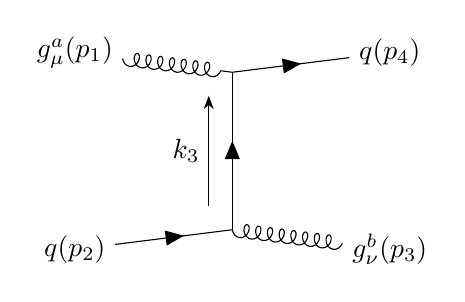
\begin{tikzpicture}[baseline={(current bounding box.center)}]
 				\begin{feynman}
 					% External Nodes
 					\vertex (i1) at (0, 2.5) {\(g^a_\mu(p_1)\)};
 					\vertex (i2) at (0, 0)   {\(q(p_2)\)};
 					\vertex (o1) at (4, 2.5) {\(q(p_4)\)};
 					\vertex (o2) at (4, 0)   {\(g^b_\nu(p_3)\)};
 					
 					% Vertices
 					\vertex (v1) at (2, 2.25);
 					\vertex (v2) at (2, 0.25);
 					
 					% Connections
 					\diagram* {
 						(i1) -- [gluon] (v1),
 						(v1) -- [fermion] (o1),
 						(i2) -- [fermion] (v2),
 						(v2) -- [gluon] (o2),
 						(v2) -- [fermion, momentum=\(k_3\)] (v1),
 					};
 				\end{feynman}
 			\end{tikzpicture}
 		\caption{canal \(u\)}
 		\end{minipage}%
 		\begin{minipage}{0.55\textwidth}
 			\centering
 			\[
 			i\mathcal{M}_u = \bar{u}(p_4) \left( ig  \gamma^\mu T^a \right ) \frac{i \slashed{k}_3}{k_3^2 + i\epsilon} \left( ig  \gamma^\nu T^b \right) u(p_2) \,\epsilon_\mu(p_1) \epsilon_\nu^*(p_3)
 			\] 			
 		\end{minipage}
 	\end{figure}
 	
 	Ainsi,en faisant les contractions pour chaque canal et en posant: \[ C^{\mu\nu\rho}(p_1, p_3, k_2)=g^{\mu \nu}(p_1 -p_3)^{\rho}+g^{\nu \rho}(p_3 -k_2)^{\mu}+g^{\rho \mu}(k_2 -p_1)^{\nu}\]
 	Nous obtenons, en explicitant les indices matricielles des générateurs 	\(T\) et en regroupant les éléments avec termes de couleurs :
 
 	\begin{equation*}
 		\begin{split}
 			i\mathcal{M}_s &= -i g^2 \, (T^b T^a)_{ji} \, \frac{1}{k_1^2+ i\epsilon} \left[ \bar{u}(p_4) \, \gamma^\nu \slashed{k}_1 \gamma^\mu \, u(p_2) \right] \epsilon_\mu(p_1) \epsilon_\nu^*(p_3) \\[1em]
 			i\mathcal{M}_t &= g^2 \, f^{abc} (T^c)_{ji} \, \frac{1}{k_2^2+ i\epsilon} \left[ \bar{u}(p_4) \, \gamma_\rho \, u(p_2) \right] C^{\mu\nu\rho}(p_1, p_3, k_2) \, \epsilon_\mu(p_1) \epsilon_\nu^*(p_3) \\[1em]
 			i\mathcal{M}_u &= -i g^2 \, (T^a T^b)_{ji} \, \frac{1}{k_3^2+ i\epsilon} \left[ \bar{u}(p_4) \, \gamma^\mu \slashed{k}_3 \gamma^\nu \, u(p_2) \right] \epsilon_\mu(p_1) \epsilon_\nu^*(p_3)
 		\end{split}
 	\end{equation*}
 	
 	Pour avoir l'amplitude réelle de l'interaction, nous utilisons:
 	\begin{equation}
 		\begin{split}
 			i\mathcal{M}=
 			&i\mathcal{M}_s + i\mathcal{M}_t + i\mathcal{M}_u \\
 			=& -i g^2 \, (T^b T^a)_{ji} \, \frac{1}{k_1^2+ i\epsilon} \left[ \bar{u}(p_4) \, \gamma^\nu \slashed{k}_1 \gamma^\mu \, u(p_2) \right] \epsilon_\mu(p_1) \epsilon_\nu^*(p_3) \\[1em]
 			 &+ g^2 \, f^{abc} (T^c)_{ji} \, \frac{1}{k_2^2+ i\epsilon} \left[ \bar{u}(p_4) \, \gamma_\rho \, u(p_2) \right] C^{\mu\nu\rho}(p_1, p_3, k_2) \, \epsilon_\mu(p_1) \epsilon_\nu^*(p_3) \\
 			 & -i g^2 \, (T^a T^b)_{ji} \, \frac{1}{k_3^2+ i\epsilon} \left[ \bar{u}(p_4) \, \gamma^\mu \slashed{k}_3 \gamma^\nu \, u(p_2) \right] \epsilon_\mu(p_1) \epsilon_\nu^*(p_3)
 		\end{split}
 	\end{equation}
 	Or, il nous a été demandé de remplacer tous les termes avec $f$ en terme $T$.\\
 	Pour cela nous utilisons la commutation entre générateurs $T$:
 	\[[T^a,T^b]=if^{abc} T^c\]
 	Cette relation se développe comme suit:
 	\[-i(T^a T^b - T^b T^a) = f^{abc} T^c \]
 	Ce qui nous donne ainsi pour l'amplitude:
 	\begin{equation}
 		\begin{split}
 			i\mathcal{M}=
 			&i\mathcal{M}_s + i\mathcal{M}_t + i\mathcal{M}_u \\
 			=& -i g^2 \, (T^b T^a)_{ji} \, \frac{1}{k_1^2+ i\epsilon} ( \bar{u}(p_4) \, \gamma^\nu \slashed{k}_1 \gamma^\mu \, u(p_2) ) \epsilon_\mu(p_1) \epsilon_\nu^*(p_3) \\[1em]
 			&+i g^2 \, (T^b T^a)_{ji} \, \frac{1}{k_2^2+ i\epsilon} ( \bar{u}(p_4) \, \gamma_\rho \, u(p_2) ) C^{\mu\nu\rho}(p_1, p_3, k_2) \, \epsilon_\mu(p_1) \epsilon_\nu^*(p_3) \\
 			&-i g^2 \, (T^a T^b)_{ji} \, \frac{1}{k_2^2+ i\epsilon} ( \bar{u}(p_4) \, \gamma_\rho \, u(p_2) ) C^{\mu\nu\rho}(p_1, p_3, k_2) \, \epsilon_\mu(p_1) \epsilon_\nu^*(p_3) \\
 			& -i g^2 \, (T^a T^b)_{ji} \, \frac{1}{k_3^2+ i\epsilon} ( \bar{u}(p_4) \, \gamma^\mu \slashed{k}_3 \gamma^\nu \, u(p_2) ) \epsilon_\mu(p_1) \epsilon_\nu^*(p_3)\\
 			=
 			&-i g^2 
 			[
 			(T^a T^b)
 			(\frac{1}{k_2^2+ i\epsilon}  (\bar{u}(p_4) \, \gamma_\rho \, u(p_2) ) C^{\mu\nu\rho}(p_1, p_3, k_2) \, \epsilon_\mu(p_1) \epsilon_\nu^*(p_3)\\
 			&+ \frac{1}{k_3^2+ i\epsilon} ( \bar{u}(p_4) \, \gamma^\mu \slashed{k}_3 \gamma^\nu \, u(p_2) ) \epsilon_\mu(p_1) \epsilon_\nu^*(p_3))\\
 			&+
 			(T^b T^a)
 			(\frac{1}{k_1^2+ i\epsilon} ( \bar{u}(p_4) \, \gamma^\nu \slashed{k}_1 \gamma^\mu \, u(p_2)) \epsilon_\mu(p_1) \epsilon_\nu^*(p_3) \\[1em]
 			&-\frac{1}{k_2^2+ i\epsilon} ( \bar{u}(p_4) \, \gamma_\rho \, u(p_2) ) C^{\mu\nu\rho}(p_1, p_3, k_2) \, \epsilon_\mu(p_1) \epsilon_\nu^*(p_3))] \\						
 		\end{split}
 	\end{equation}
 	
 	On peut poser:
 	\begin{equation}
 		\begin{split}
	 		A&=\frac{1}{k_2^2+ i\epsilon}  (\bar{u}(p_4) \, \gamma_\rho \, u(p_2) ) C^{\mu\nu\rho}(p_1, p_3, k_2) \, \epsilon_\mu(p_1) \epsilon_\nu^*(p_3)\\
	 		B&=\frac{1}{k_3^2+ i\epsilon} ( \bar{u}(p_4) \, \gamma^\mu \slashed{k}_3 \gamma^\nu \, u(p_2) ) \epsilon_\mu(p_1) \epsilon_\nu^*(p_3) \\
	 		C&=\frac{1}{k_1^2+ i\epsilon} ( \bar{u}(p_4) \, \gamma^\nu \slashed{k}_1 \gamma^\mu \, u(p_2)) \epsilon_\mu(p_1) \epsilon_\nu^*(p_3) \\
	 		D&=\frac{1}{k_2^2+ i\epsilon} ( \bar{u}(p_4) \, \gamma_\rho \, u(p_2) ) C^{\mu\nu\rho}(p_1, p_3, k_2) \, \epsilon_\mu(p_1) \epsilon_\nu^*(p_3)
 		\end{split}
 	\end{equation}
 	Ce qui nous donne:
 	\fbox{\(\mathcal{M}(q+g \rightarrow q+g)= -ig^2 [(T^a T^b)(A+B)+(T^b T^A)(C-D)]\)}
 	\nocite{*}
 	\bibliographystyle{plain}
 	\bibliography{biblioquarkgluonscattering}
 \end{document}
 	
 		
 
 